\documentclass[border={0.5cm 0.5cm 0.5cm 1cm}]{standalone}  %E,S,W,N

\usepackage{amssymb}
\usepackage{amsmath}
\usepackage{tikz}
\usepackage{pgfplots}
\pgfplotsset{compat=1.13}
\usepgfplotslibrary{polar}	%for spirals
\frenchspacing

\begin{document}
	
	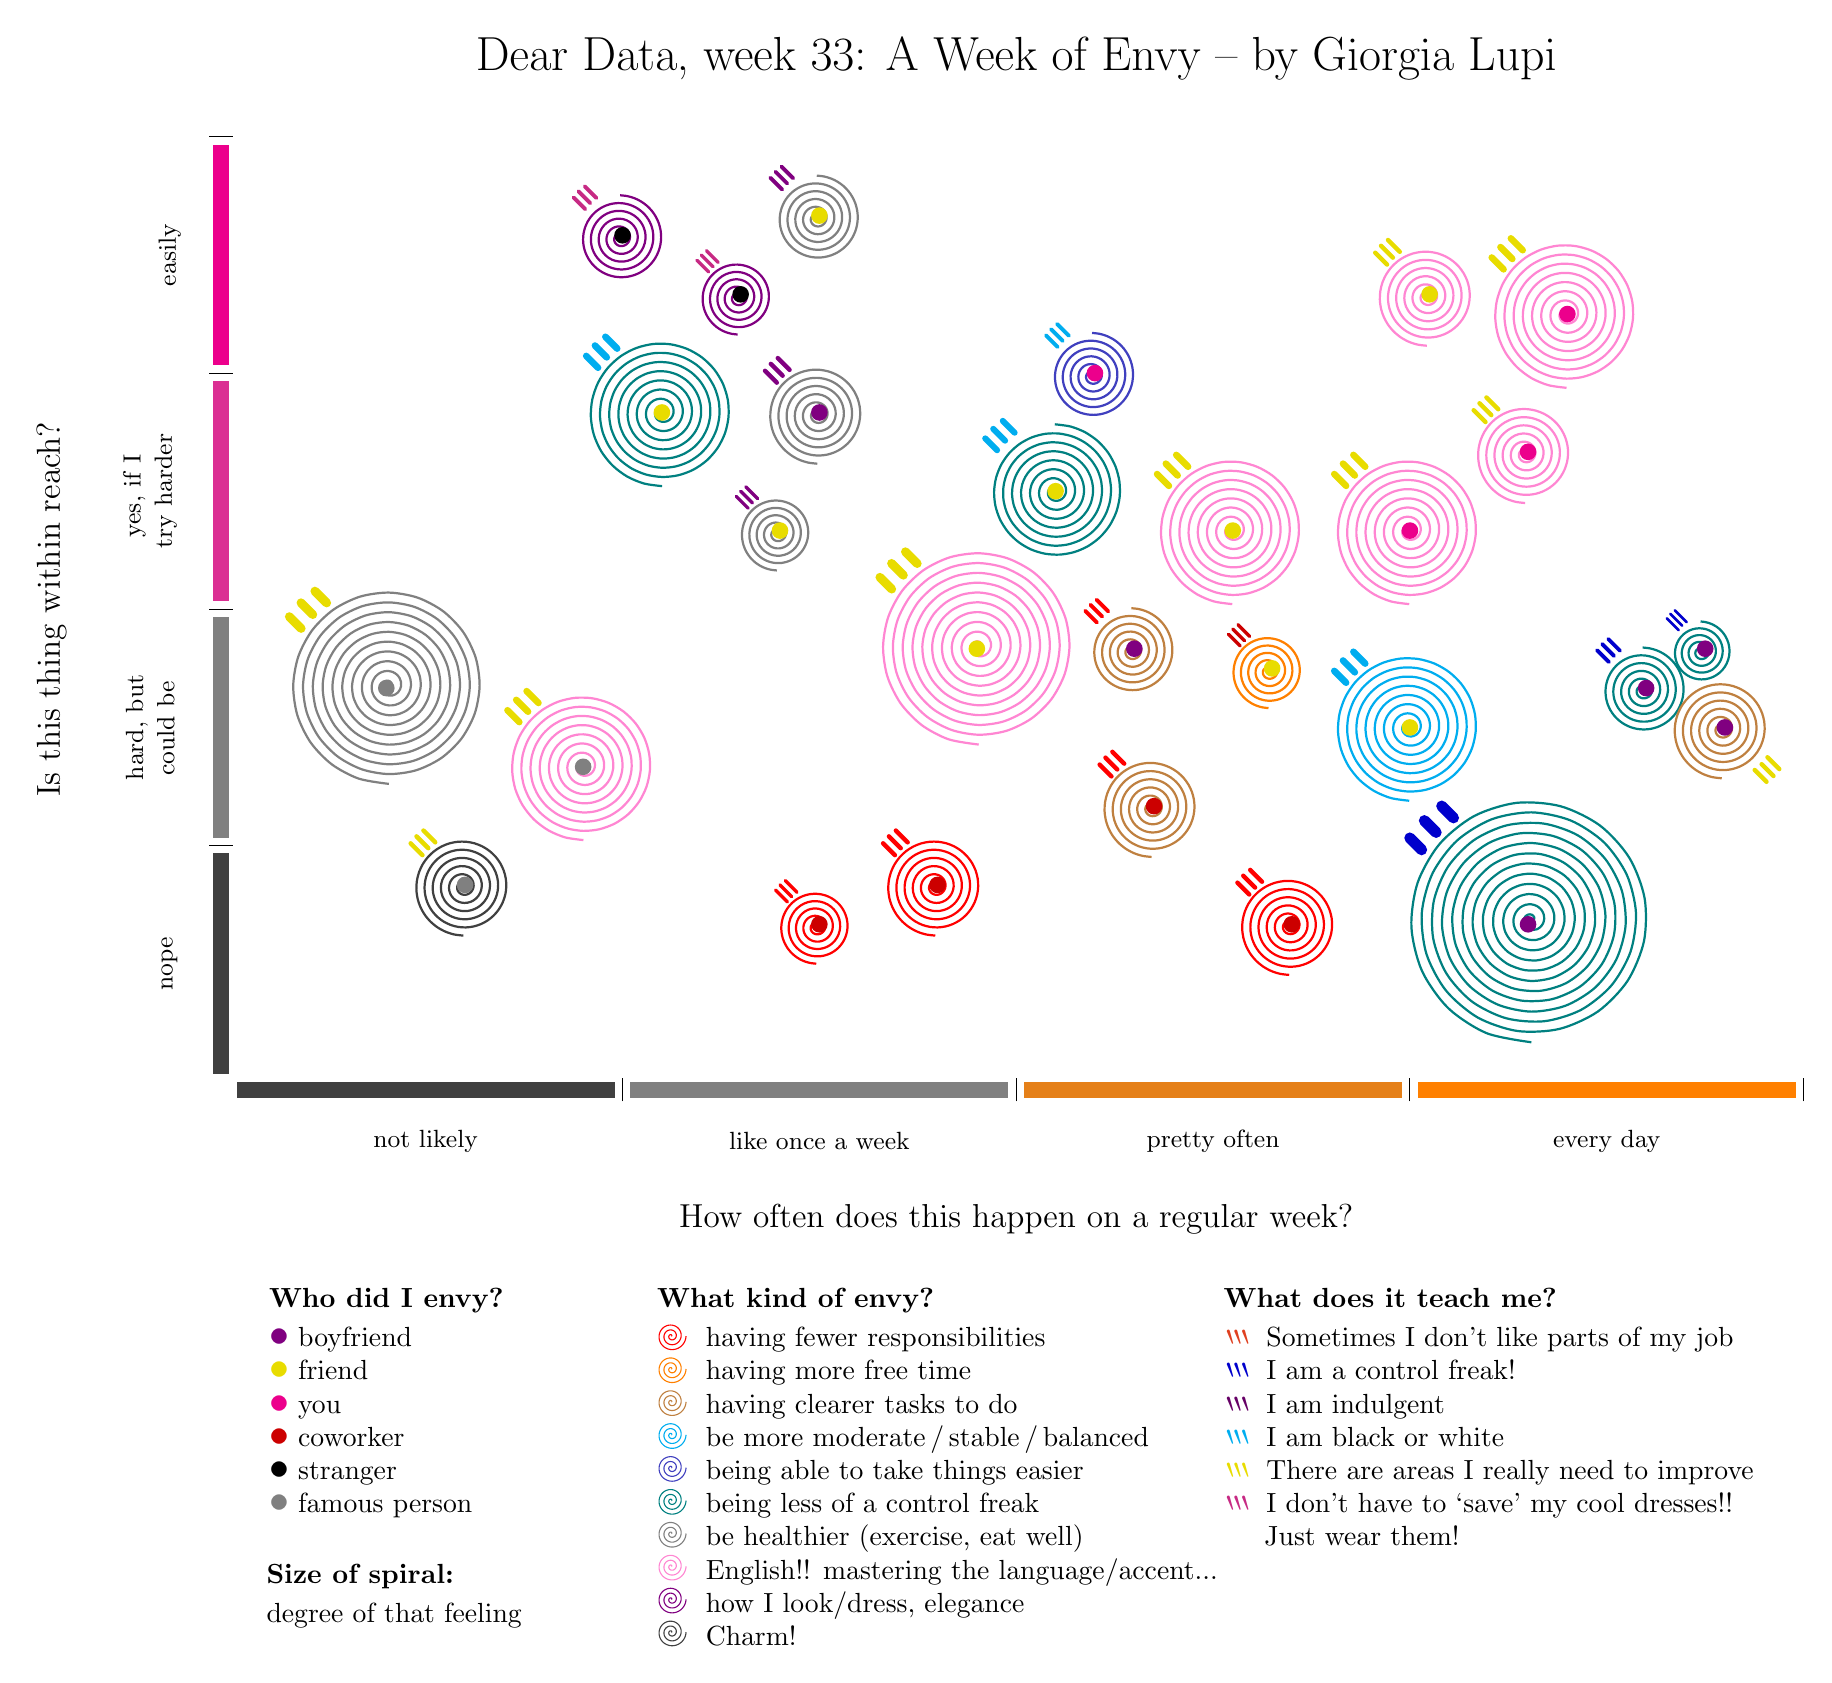
\begin{tikzpicture}	
	\def\y{12}	%height of y-axis -- if axis is multiple of 4, ticks match grid lines
	\def\x{20}	%width of x-axis
	\node at (\x/2,\y+1) {\LARGE Dear Data, week 33: A Week of Envy -- by Giorgia Lupi};
	
	%Y-AXIS
	\node at (-2.25,\y/2) {\rotatebox{90}{\large Is this thing within reach?}};
	\foreach \i [count=\c from 0] in {darkgray,gray,magenta!80!gray,magenta}{
		\fill[\i] (0,\c*\y/4+0.1) rectangle (-0.2,{(\c+1)*\y/4-0.1});
		\draw (-0.25,{(\c+1)*\y/4})--++(0.3,0);
	}
	\node at (-0.75,0.25*\y/2+0*\y/4) {\rotatebox{90}{\small nope}};
	\node at (-1.00,0.25*\y/2+1*\y/4) {\rotatebox{90}{\small hard, but} \\[0.35mm] 
									   \rotatebox{90}{\small $\,$could be}};
	\node at (-1.00,0.25*\y/2+2*\y/4) {\rotatebox{90}{\small $\;\,$yes, if I} \\[0.35mm]
									   \rotatebox{90}{\small try harder}};
	\node at (-0.75,0.25*\y/2+3*\y/4) {\rotatebox{90}{\small easily}};
	
	%X-AXIS
	\node at (\x/2,-1.75) {\large How often does this happen on a regular week?};
	\foreach \i [count=\c from 0] in {darkgray,gray,orange!80!gray,orange}{
		\fill[\i] (\c*\x/4+0.1,0) rectangle ({(\c+1)*\x/4-0.1},-0.2);
		\draw ({(\c+1)*\x/4},-0.25)--++(0,0.3);
	}
	\node at (0.5*\x/4+0*\x/4,-0.75) {\small not likely};
	\node at (0.5*\x/4+1*\x/4,-0.75) {\small like once a week};
	\node at (0.5*\x/4+2*\x/4,-0.75) {\small pretty often};
	\node at (0.5*\x/4+3*\x/4,-0.75) {\small every day};
	
	%LEGEND
	%WHO DID I ENVY?
	\node[align=left,below] at (0.1*\x,-2.5) {\bfseries Who did I envy?\\[0.75mm]
					  {\Large\color{violet} $\bullet$} boyfriend\\
					  {\Large\color{yellow!80!olive} $\bullet$} friend\\
					  {\Large\color{magenta} $\bullet$} you\\
					  {\Large\color{red!80!black} $\bullet$} coworker\\
					  {\Large\color{black} $\bullet$} stranger\\
					  {\Large\color{gray} $\bullet$} famous person\\
					  };
	\node[align=left,below] at (0.1*\x+0.1,-6) {\bfseries Size of spiral: \\[0.75mm]
		degree of that feeling};
	
	%WHAT KIND OF ENVY?
	\def\kindx{0.45*\x}
	\node[align=left,below] at (\kindx,-2.5) {\bfseries What kind of envy?\\[0.75mm]
		\hspace{0.5cm} having fewer responsibilities\\
		\hspace{0.5cm} having more free time\\
		\hspace{0.5cm} having clearer tasks to do\\
		\hspace{0.5cm} be more moderate$\,$/$\,$stable$\,$/$\,$balanced\\
		\hspace{0.5cm} being able to take things easier\\
		\hspace{0.5cm} being less of a control freak\\
		\hspace{0.5cm} be healthier (exercise, eat well)\\
		\hspace{0.5cm} English!! mastering the language/accent...\\
		\hspace{0.5cm} how I look/dress, elegance\\
		\hspace{0.5cm} Charm!
	};
	\foreach \i [count=\c from 0] in {red,orange,brown,cyan,blue!50!gray,teal,gray,pink!70!magenta,violet,darkgray} {		\begin{polaraxis}[axis lines=none,no marks,samples=201,smooth,domain=0:3, xshift={-2-9*0.06+29*0.6*\kindx},yshift={-2-9*0.06-29*0.98*3.35-29*0.41*\c},scale=0.06,color=blue]
	\addplot+[\i] (2*180*x,x);
	\end{polaraxis}
	}
	%TO DO: horizontal spiral placement doesn't update correctly when \kindx changes -- fix this
	%TODO	if I update \kindx from 0.45 to 0.5, need to update 0.6*\kindx to 0.65*\kindx, etc.
	
	%WHAT DOES IT TEACH ME?
	\node[align=left,below] at (0.8*\x,-2.5) {\bfseries What does it teach me?\\[0.75mm]
	{\LARGE\color{red!50!brown} \reflectbox{$\,_{'''}$}} Sometimes I don't like parts of my job\\
	{\LARGE\color{blue!80!black} \reflectbox{$\,_{'''}$}} I am a control freak!\\
	{\LARGE\color{violet!80!black} \reflectbox{$\,_{'''}$}} I am indulgent\\
	{\LARGE\color{cyan} \reflectbox{$\,_{'''}$}} I am black or white\\
	{\LARGE\color{yellow!80!olive} \reflectbox{$\,_{'''}$}} There are areas I really need to improve\\
	{\LARGE\color{magenta!80!black} \reflectbox{$\,_{'''}$}} I don't have to `save' my cool dresses!!\\
											  				\hspace{0.4cm} Just wear them!
	};
	
%------------------------------------------------------------------------------------------
	%SPIRALS -- replicating original, going left-to-right, down-to-up
%------------------------------------------ 
%------------------------------------------ LOWER LEFT
	\begin{scope}
	\def\sx{2}		\def\sy{5}		%horizontal length, vertical height of spiral
	\def\size{4} 						%scaling -- from 2 to 5
	\def\dotcolor{gray}		\def\spiralcolor{gray}		\def\tickcolor{yellow!80!olive}
	\begin{polaraxis}[axis lines=none,no marks,samples=201,smooth,domain=0:4, xshift={-2-9*\size+29*0.98*\sx},yshift={-2-9*\size+29*0.98*\sy},scale=0.1*\size,rotate=-90]
	\addplot+[\spiralcolor,thick] ({(\size+1)*180*x},x);
	\end{polaraxis}	
	\foreach \i in {125,135,145} \draw[\tickcolor,line width=0.8*\size,line cap=round] ({\sx+0.33*\size*cos(\i)},{\sy+0.33*\size*sin(\i)})--++(-0.15,0.15); %ticks
	\fill[\dotcolor] (\sx,\sy) circle (3pt);	%dot in center
	\end{scope}
%------------------------------------------
	\begin{scope}
	\def\sx{3}		\def\sy{2.5}		%horizontal length, vertical height of spiral
	\def\size{2} 						%scaling -- from 2 to 5
	\def\dotcolor{gray}		\def\spiralcolor{darkgray}		\def\tickcolor{yellow!80!olive}
	\begin{polaraxis}[axis lines=none,no marks,samples=201,smooth,domain=0:4, xshift={-2-9*\size+29*0.98*\sx},yshift={-2-9*\size+29*0.98*\sy},scale=0.1*\size,rotate=-90]
	\addplot+[\spiralcolor,thick] ({(\size+1)*180*x},x);
	\end{polaraxis}	
	\foreach \i in {125,135,145} \draw[\tickcolor,line width=0.8*\size,line cap=round] ({\sx+0.33*\size*cos(\i)},{\sy+0.33*\size*sin(\i)})--++(-0.15,0.15); %ticks
	\fill[\dotcolor] (\sx,\sy) circle (3pt);	%dot in center
	\end{scope}
%------------------------------------------	
	\begin{scope}
	\def\sx{4.5}		\def\sy{4}		%horizontal length, vertical height of spiral
	\def\size{3} 						%scaling -- from 2 to 5
	\def\dotcolor{gray}		\def\spiralcolor{pink!70!magenta}	\def\tickcolor{yellow!80!olive}
	\begin{polaraxis}[axis lines=none,no marks,samples=201,smooth,domain=0:4, xshift={-2-9*\size+29*0.98*\sx},yshift={-2-9*\size+29*0.98*\sy},scale=0.1*\size,rotate=-90]
	\addplot+[\spiralcolor,thick] ({(\size+1)*180*x},x);
	\end{polaraxis}	
	\foreach \i in {125,135,145} \draw[\tickcolor,line width=0.8*\size,line cap=round] ({\sx+0.33*\size*cos(\i)},{\sy+0.33*\size*sin(\i)})--++(-0.15,0.15); %ticks
	\fill[\dotcolor] (\sx,\sy) circle (3pt);	%dot in center
	\end{scope}
%------------------------------------------	
%------------------------------------------	UPPER LEFT
	\begin{scope}
	\def\sx{7}		\def\sy{7}	%horizontal length, vertical height of spiral
	\def\size{1.5} 						%scaling -- from 2 to 5
	\def\dotcolor{yellow!80!olive}		\def\spiralcolor{gray}	\def\tickcolor{violet}
	\begin{polaraxis}[axis lines=none,no marks,samples=201,smooth,domain=0:4, xshift={-2-9*\size+29*0.98*\sx},yshift={-2-9*\size+29*0.98*\sy},scale=0.1*\size,rotate=-90]
	\addplot+[\spiralcolor,thick] ({(\size+1)*180*x},x);
	\end{polaraxis}	
	\foreach \i in {125,135,145} \draw[\tickcolor,line width=0.8*\size,line cap=round] ({\sx+0.33*\size*cos(\i)},{\sy+0.33*\size*sin(\i)})--++(-0.15,0.15); %ticks
	\fill[\dotcolor] (\sx,\sy) circle (3pt);	%dot in center
	\end{scope}
%------------------------------------------	
	\begin{scope}
	\def\sx{5.5}		\def\sy{8.5}		%horizontal length, vertical height of spiral
	\def\size{3} 						%scaling -- from 2 to 5
	\def\dotcolor{yellow!80!olive}		\def\spiralcolor{teal}	\def\tickcolor{cyan}
	\begin{polaraxis}[axis lines=none,no marks,samples=201,smooth,domain=0:4, xshift={-2-9*\size+29*0.98*\sx},yshift={-2-9*\size+29*0.98*\sy},scale=0.1*\size,rotate=-90]
	\addplot+[\spiralcolor,thick] ({(\size+1)*180*x},x);
	\end{polaraxis}	
	\foreach \i in {125,135,145} \draw[\tickcolor,line width=0.8*\size,line cap=round] ({\sx+0.33*\size*cos(\i)},{\sy+0.33*\size*sin(\i)})--++(-0.15,0.15); %ticks
	\fill[\dotcolor] (\sx,\sy) circle (3pt);	%dot in center
	\end{scope}
%------------------------------------------	
	\begin{scope}
	\def\sx{7.5}		\def\sy{8.5}	%horizontal length, vertical height of spiral
	\def\size{2} 						%scaling -- from 2 to 5
	\def\dotcolor{violet}		\def\spiralcolor{gray}	\def\tickcolor{violet}
	\begin{polaraxis}[axis lines=none,no marks,samples=201,smooth,domain=0:4, xshift={-2-9*\size+29*0.98*\sx},yshift={-2-9*\size+29*0.98*\sy},scale=0.1*\size,rotate=-90]
	\addplot+[\spiralcolor,thick] ({(\size+1)*180*x},x);
	\end{polaraxis}	
	\foreach \i in {125,135,145} \draw[\tickcolor,line width=0.8*\size,line cap=round] ({\sx+0.33*\size*cos(\i)},{\sy+0.33*\size*sin(\i)})--++(-0.15,0.15); %ticks
	\fill[\dotcolor] (\sx,\sy) circle (3pt);	%dot in center
	\end{scope}
%------------------------------------------	
	\begin{scope}
	\def\sx{6.5}		\def\sy{10}	%horizontal length, vertical height of spiral
	\def\size{1.5} 						%scaling -- from 2 to 5
	\def\dotcolor{black}	\def\spiralcolor{violet}	\def\tickcolor{magenta!80!black}
	\begin{polaraxis}[axis lines=none,no marks,samples=201,smooth,domain=0:4, xshift={-2-9*\size+29*0.98*\sx},yshift={-2-9*\size+29*0.98*\sy},scale=0.1*\size,rotate=-90]
	\addplot+[\spiralcolor,thick] ({(\size+1)*180*x},x);
	\end{polaraxis}	
	\foreach \i in {125,135,145} \draw[\tickcolor,line width=0.8*\size,line cap=round] ({\sx+0.33*\size*cos(\i)},{\sy+0.33*\size*sin(\i)})--++(-0.15,0.15); %ticks
	\fill[\dotcolor] (\sx,\sy) circle (3pt);	%dot in center
	\end{scope}
%------------------------------------------	
	\begin{scope}
	\def\sx{5}		\def\sy{10.75}	%horizontal length, vertical height of spiral
	\def\size{1.75} 						%scaling -- from 2 to 5
	\def\dotcolor{black}	\def\spiralcolor{violet}	\def\tickcolor{magenta!80!black}
	\begin{polaraxis}[axis lines=none,no marks,samples=201,smooth,domain=0:4, xshift={-2-9*\size+29*0.98*\sx},yshift={-2-9*\size+29*0.98*\sy},scale=0.1*\size,rotate=-90]
	\addplot+[\spiralcolor,thick] ({(\size+1)*180*x},x);
	\end{polaraxis}	
	\foreach \i in {125,135,145} \draw[\tickcolor,line width=0.8*\size,line cap=round] ({\sx+0.33*\size*cos(\i)},{\sy+0.33*\size*sin(\i)})--++(-0.15,0.15); %ticks
	\fill[\dotcolor] (\sx,\sy) circle (3pt);	%dot in center
	\end{scope}
%------------------------------------------	
	\begin{scope}
	\def\sx{7.5}		\def\sy{11}	%horizontal length, vertical height of spiral
	\def\size{1.75} 						%scaling -- from 2 to 5
	\def\dotcolor{yellow!80!olive}	\def\spiralcolor{gray}	\def\tickcolor{violet}
	\begin{polaraxis}[axis lines=none,no marks,samples=201,smooth,domain=0:4, xshift={-2-9*\size+29*0.98*\sx},yshift={-2-9*\size+29*0.98*\sy},scale=0.1*\size,rotate=-90]
	\addplot+[\spiralcolor,thick] ({(\size+1)*180*x},x);
	\end{polaraxis}	
	\foreach \i in {125,135,145} \draw[\tickcolor,line width=0.8*\size,line cap=round] ({\sx+0.33*\size*cos(\i)},{\sy+0.33*\size*sin(\i)})--++(-0.15,0.15); %ticks
	\fill[\dotcolor] (\sx,\sy) circle (3pt);	%dot in center
	\end{scope}
%------------------------------------------	
%------------------------------------------	MIDDLE PART
	\begin{scope}
	\def\sx{7.5}		\def\sy{2}	%horizontal length, vertical height of spiral
	\def\size{1.5} 						%scaling -- from 2 to 5
	\def\dotcolor{red!80!black}		\def\spiralcolor{red}	\def\tickcolor{red}
	\begin{polaraxis}[axis lines=none,no marks,samples=201,smooth,domain=0:4, xshift={-2-9*\size+29*0.98*\sx},yshift={-2-9*\size+29*0.98*\sy},scale=0.1*\size,rotate=-90]
	\addplot+[\spiralcolor,thick] ({(\size+1)*180*x},x);
	\end{polaraxis}	
	\foreach \i in {125,135,145} \draw[\tickcolor,line width=0.8*\size,line cap=round] ({\sx+0.33*\size*cos(\i)},{\sy+0.33*\size*sin(\i)})--++(-0.15,0.15); %ticks
	\fill[\dotcolor] (\sx,\sy) circle (3pt);	%dot in center
	\end{scope}
%------------------------------------------	
	\begin{scope}
	\def\sx{9}		\def\sy{2.5}	%horizontal length, vertical height of spiral
	\def\size{2} 						%scaling -- from 2 to 5
	\def\dotcolor{red!80!black}		\def\spiralcolor{red}	\def\tickcolor{red}
	\begin{polaraxis}[axis lines=none,no marks,samples=201,smooth,domain=0:4, xshift={-2-9*\size+29*0.98*\sx},yshift={-2-9*\size+29*0.98*\sy},scale=0.1*\size,rotate=-90]
	\addplot+[\spiralcolor,thick] ({(\size+1)*180*x},x);
	\end{polaraxis}	
	\foreach \i in {125,135,145} \draw[\tickcolor,line width=0.8*\size,line cap=round] ({\sx+0.33*\size*cos(\i)},{\sy+0.33*\size*sin(\i)})--++(-0.15,0.15); %ticks
	\fill[\dotcolor] (\sx,\sy) circle (3pt);	%dot in center
	\end{scope}
%------------------------------------------	
	\begin{scope}
	\def\sx{11.75}		\def\sy{3.5}	%horizontal length, vertical height of spiral
	\def\size{2} 						%scaling -- from 2 to 5
	\def\dotcolor{red!80!black}		\def\spiralcolor{brown}	\def\tickcolor{red}
	\begin{polaraxis}[axis lines=none,no marks,samples=201,smooth,domain=0:4, xshift={-2-9*\size+29*0.98*\sx},yshift={-2-9*\size+29*0.98*\sy},scale=0.1*\size,rotate=-90]
	\addplot+[\spiralcolor,thick] ({(\size+1)*180*x},x);
	\end{polaraxis}	
	\foreach \i in {125,135,145} \draw[\tickcolor,line width=0.8*\size,line cap=round] ({\sx+0.33*\size*cos(\i)},{\sy+0.33*\size*sin(\i)})--++(-0.15,0.15); %ticks
	\fill[\dotcolor] (\sx,\sy) circle (3pt);	%dot in center
	\end{scope}
%------------------------------------------	
	\begin{scope}
	\def\sx{13.5}		\def\sy{2}	%horizontal length, vertical height of spiral
	\def\size{2} 						%scaling -- from 2 to 5
	\def\dotcolor{red!80!black}		\def\spiralcolor{red}	\def\tickcolor{red}
	\begin{polaraxis}[axis lines=none,no marks,samples=201,smooth,domain=0:4, xshift={-2-9*\size+29*0.98*\sx},yshift={-2-9*\size+29*0.98*\sy},scale=0.1*\size,rotate=-90]
	\addplot+[\spiralcolor,thick] ({(\size+1)*180*x},x);
	\end{polaraxis}	
	\foreach \i in {125,135,145} \draw[\tickcolor,line width=0.8*\size,line cap=round] ({\sx+0.33*\size*cos(\i)},{\sy+0.33*\size*sin(\i)})--++(-0.15,0.15); %ticks
	\fill[\dotcolor] (\sx,\sy) circle (3pt);	%dot in center
	\end{scope}
%------------------------------------------	
	\begin{scope}
	\def\sx{11.5}		\def\sy{5.5}	%horizontal length, vertical height of spiral
	\def\size{1.75} 						%scaling -- from 2 to 5
	\def\dotcolor{violet}		\def\spiralcolor{brown}	\def\tickcolor{red}
	\begin{polaraxis}[axis lines=none,no marks,samples=201,smooth,domain=0:4, xshift={-2-9*\size+29*0.98*\sx},yshift={-2-9*\size+29*0.98*\sy},scale=0.1*\size,rotate=-90]
	\addplot+[\spiralcolor,thick] ({(\size+1)*180*x},x);
	\end{polaraxis}	
	\foreach \i in {125,135,145} \draw[\tickcolor,line width=0.8*\size,line cap=round] ({\sx+0.33*\size*cos(\i)},{\sy+0.33*\size*sin(\i)})--++(-0.15,0.15); %ticks
	\fill[\dotcolor] (\sx,\sy) circle (3pt);	%dot in center
	\end{scope}
%------------------------------------------	
	\begin{scope}
	\def\sx{9.5}		\def\sy{5.5}		%horizontal length, vertical height of spiral
	\def\size{4} 						%scaling -- from 2 to 5
	\def\dotcolor{yellow!80!olive}	\def\spiralcolor{pink!70!magenta}	\def\tickcolor{yellow!80!olive}
	\begin{polaraxis}[axis lines=none,no marks,samples=201,smooth,domain=0:4, xshift={-2-9*\size+29*0.98*\sx},yshift={-2-9*\size+29*0.98*\sy},scale=0.1*\size,rotate=-90]
	\addplot+[\spiralcolor,thick] ({(\size+1)*180*x},x);
	\end{polaraxis}	
	\foreach \i in {125,135,145} \draw[\tickcolor,line width=0.8*\size,line cap=round] ({\sx+0.33*\size*cos(\i)},{\sy+0.33*\size*sin(\i)})--++(-0.15,0.15); %ticks
	\fill[\dotcolor] (\sx,\sy) circle (3pt);	%dot in center
	\end{scope}
%------------------------------------------	
	\begin{scope}
	\def\sx{10.5}		\def\sy{7.5}	%horizontal length, vertical height of spiral
	\def\size{2.75} 						%scaling -- from 2 to 5
	\def\dotcolor{yellow!80!olive}		\def\spiralcolor{teal}	\def\tickcolor{cyan}
	\begin{polaraxis}[axis lines=none,no marks,samples=201,smooth,domain=0:4, xshift={-2-9*\size+29*0.98*\sx},yshift={-2-9*\size+29*0.98*\sy},scale=0.1*\size,rotate=-90]
	\addplot+[\spiralcolor,thick] ({(\size+1)*180*x},x);
	\end{polaraxis}	
	\foreach \i in {125,135,145} \draw[\tickcolor,line width=0.8*\size,line cap=round] ({\sx+0.33*\size*cos(\i)},{\sy+0.33*\size*sin(\i)})--++(-0.15,0.15); %ticks
	\fill[\dotcolor] (\sx,\sy) circle (3pt);	%dot in center
	\end{scope}
%------------------------------------------	
	\begin{scope}
	\def\sx{11}		\def\sy{9}	%horizontal length, vertical height of spiral
	\def\size{1.75} 						%scaling -- from 2 to 5
	\def\dotcolor{magenta}		\def\spiralcolor{blue!50!gray}	\def\tickcolor{cyan}
	\begin{polaraxis}[axis lines=none,no marks,samples=201,smooth,domain=0:4, xshift={-2-9*\size+29*0.98*\sx},yshift={-2-9*\size+29*0.98*\sy},scale=0.1*\size,rotate=-90]
	\addplot+[\spiralcolor,thick] ({(\size+1)*180*x},x);
	\end{polaraxis}	
	\foreach \i in {125,135,145} \draw[\tickcolor,line width=0.8*\size,line cap=round] ({\sx+0.33*\size*cos(\i)},{\sy+0.33*\size*sin(\i)})--++(-0.15,0.15); %ticks
	\fill[\dotcolor] (\sx,\sy) circle (3pt);	%dot in center
	\end{scope}
%------------------------------------------	
%------------------------------------------	RIGHT SIDE
	\begin{scope}
	\def\sx{16.5}		\def\sy{2}			%horizontal length, vertical height of spiral
	\def\size{5} 						%scaling -- from 2 to 5
	\def\dotcolor{violet}		\def\spiralcolor{teal}		\def\tickcolor{blue!80!black}
	\begin{polaraxis}[axis lines=none,no marks,samples=201,smooth,domain=0:4, xshift={-2-9*\size+29*0.98*\sx},yshift={-2-9*\size+29*0.98*\sy},scale=0.1*\size,rotate=-90]
	\addplot+[\spiralcolor,thick] ({(\size+1)*180*x},x);
	\end{polaraxis}	
	\foreach \i in {125,135,145} \draw[\tickcolor,line width=0.8*\size,line cap=round] ({\sx+0.33*\size*cos(\i)},{\sy+0.33*\size*sin(\i)})--++(-0.15,0.15); %ticks
	\fill[\dotcolor] (\sx,\sy) circle (3pt);	%dot in center
	\end{scope}
%------------------------------------------	
	\begin{scope}
	\def\sx{15}		\def\sy{4.5}		%horizontal length, vertical height of spiral
	\def\size{3} 						%scaling -- from 2 to 5
	\def\dotcolor{yellow!80!olive}		\def\spiralcolor{cyan}		\def\tickcolor{cyan}
	\begin{polaraxis}[axis lines=none,no marks,samples=201,smooth,domain=0:4, xshift={-2-9*\size+29*0.98*\sx},yshift={-2-9*\size+29*0.98*\sy},scale=0.1*\size,rotate=-90]
	\addplot+[\spiralcolor,thick] ({(\size+1)*180*x},x);
	\end{polaraxis}	
	\foreach \i in {125,135,145} \draw[\tickcolor,line width=0.8*\size,line cap=round] ({\sx+0.33*\size*cos(\i)},{\sy+0.33*\size*sin(\i)})--++(-0.15,0.15); %ticks
	\fill[\dotcolor] (\sx,\sy) circle (3pt);	%dot in center
	\end{scope}
%------------------------------------------	
	\begin{scope}
	\def\sx{13.25}		\def\sy{5.25}		%horizontal length, vertical height of spiral
	\def\size{1.5} 						%scaling -- from 2 to 5
	\def\dotcolor{yellow!80!olive}		\def\spiralcolor{orange}		\def\tickcolor{red!80!black}
	\begin{polaraxis}[axis lines=none,no marks,samples=201,smooth,domain=0:4, xshift={-2-9*\size+29*0.98*\sx},yshift={-2-9*\size+29*0.98*\sy},scale=0.1*\size,rotate=-90]
	\addplot+[\spiralcolor,thick] ({(\size+1)*180*x},x);
	\end{polaraxis}	
	\foreach \i in {125,135,145} \draw[\tickcolor,line width=0.8*\size,line cap=round] ({\sx+0.33*\size*cos(\i)},{\sy+0.33*\size*sin(\i)})--++(-0.15,0.15); %ticks
	\fill[\dotcolor] (\sx,\sy) circle (3pt);	%dot in center
	\end{scope}
%------------------------------------------	
	\begin{scope}
	\def\sx{12.75}		\def\sy{7}		%horizontal length, vertical height of spiral
	\def\size{3} 						%scaling -- from 2 to 5
	\def\dotcolor{yellow!80!olive}	\def\spiralcolor{pink!70!magenta}	\def\tickcolor{yellow!80!olive}
	\begin{polaraxis}[axis lines=none,no marks,samples=201,smooth,domain=0:4, xshift={-2-9*\size+29*0.98*\sx},yshift={-2-9*\size+29*0.98*\sy},scale=0.1*\size,rotate=-90]
	\addplot+[\spiralcolor,thick] ({(\size+1)*180*x},x);
	\end{polaraxis}	
	\foreach \i in {125,135,145} \draw[\tickcolor,line width=0.8*\size,line cap=round] ({\sx+0.33*\size*cos(\i)},{\sy+0.33*\size*sin(\i)})--++(-0.15,0.15); %ticks
	\fill[\dotcolor] (\sx,\sy) circle (3pt);	%dot in center
	\end{scope}
%------------------------------------------	
	\begin{scope}
	\def\sx{15}		\def\sy{7}		%horizontal length, vertical height of spiral
	\def\size{3} 						%scaling -- from 2 to 5
	\def\dotcolor{magenta}	\def\spiralcolor{pink!70!magenta}	\def\tickcolor{yellow!80!olive}
	\begin{polaraxis}[axis lines=none,no marks,samples=201,smooth,domain=0:4, xshift={-2-9*\size+29*0.98*\sx},yshift={-2-9*\size+29*0.98*\sy},scale=0.1*\size,rotate=-90]
	\addplot+[\spiralcolor,thick] ({(\size+1)*180*x},x);
	\end{polaraxis}	
	\foreach \i in {125,135,145} \draw[\tickcolor,line width=0.8*\size,line cap=round] ({\sx+0.33*\size*cos(\i)},{\sy+0.33*\size*sin(\i)})--++(-0.15,0.15); %ticks
	\fill[\dotcolor] (\sx,\sy) circle (3pt);	%dot in center
	\end{scope}
%------------------------------------------	
	\begin{scope}
	\def\sx{16.5}		\def\sy{8}		%horizontal length, vertical height of spiral
	\def\size{2} 						%scaling -- from 2 to 5
	\def\dotcolor{magenta}	\def\spiralcolor{pink!70!magenta}	\def\tickcolor{yellow!80!olive}
	\begin{polaraxis}[axis lines=none,no marks,samples=201,smooth,domain=0:4, xshift={-2-9*\size+29*0.98*\sx},yshift={-2-9*\size+29*0.98*\sy},scale=0.1*\size,rotate=-90]
	\addplot+[\spiralcolor,thick] ({(\size+1)*180*x},x);
	\end{polaraxis}	
	\foreach \i in {125,135,145} \draw[\tickcolor,line width=0.8*\size,line cap=round] ({\sx+0.33*\size*cos(\i)},{\sy+0.33*\size*sin(\i)})--++(-0.15,0.15); %ticks
	\fill[\dotcolor] (\sx,\sy) circle (3pt);	%dot in center
	\end{scope}
%------------------------------------------	
	\begin{scope}
	\def\sx{15.25}		\def\sy{10}		%horizontal length, vertical height of spiral
	\def\size{2} 						%scaling -- from 2 to 5
	\def\dotcolor{yellow!80!olive}	\def\spiralcolor{pink!70!magenta}	\def\tickcolor{yellow!80!olive}
	\begin{polaraxis}[axis lines=none,no marks,samples=201,smooth,domain=0:4, xshift={-2-9*\size+29*0.98*\sx},yshift={-2-9*\size+29*0.98*\sy},scale=0.1*\size,rotate=-90]
	\addplot+[\spiralcolor,thick] ({(\size+1)*180*x},x);
	\end{polaraxis}	
	\foreach \i in {125,135,145} \draw[\tickcolor,line width=0.8*\size,line cap=round] ({\sx+0.33*\size*cos(\i)},{\sy+0.33*\size*sin(\i)})--++(-0.15,0.15); %ticks
	\fill[\dotcolor] (\sx,\sy) circle (3pt);	%dot in center
	\end{scope}
%------------------------------------------	
	\begin{scope}
	\def\sx{17}		\def\sy{9.75}		%horizontal length, vertical height of spiral
	\def\size{3} 						%scaling -- from 2 to 5
	\def\dotcolor{magenta}	\def\spiralcolor{pink!70!magenta}	\def\tickcolor{yellow!80!olive}
	\begin{polaraxis}[axis lines=none,no marks,samples=201,smooth,domain=0:4, xshift={-2-9*\size+29*0.98*\sx},yshift={-2-9*\size+29*0.98*\sy},scale=0.1*\size,rotate=-90]
	\addplot+[\spiralcolor,thick] ({(\size+1)*180*x},x);
	\end{polaraxis}	
	\foreach \i in {125,135,145} \draw[\tickcolor,line width=0.8*\size,line cap=round] ({\sx+0.33*\size*cos(\i)},{\sy+0.33*\size*sin(\i)})--++(-0.15,0.15); %ticks
	\fill[\dotcolor] (\sx,\sy) circle (3pt);	%dot in center
	\end{scope}
%------------------------------------------	
%------------------------------------------	%LOWER RIGHT
	\begin{scope}
	\def\sx{18}		\def\sy{5}			%horizontal length, vertical height of spiral
	\def\size{1.75} 						%scaling -- from 2 to 5
	\def\dotcolor{violet}		\def\spiralcolor{teal}		\def\tickcolor{blue!80!black}
	\begin{polaraxis}[axis lines=none,no marks,samples=201,smooth,domain=0:4, xshift={-2-9*\size+29*0.98*\sx},yshift={-2-9*\size+29*0.98*\sy},scale=0.1*\size,rotate=-90]
	\addplot+[\spiralcolor,thick] ({(\size+1)*180*x},x);
	\end{polaraxis}	
	\foreach \i in {125,135,145} \draw[\tickcolor,line width=0.8*\size,line cap=round] ({\sx+0.33*\size*cos(\i)},{\sy+0.33*\size*sin(\i)})--++(-0.15,0.15); %ticks
	\fill[\dotcolor] (\sx,\sy) circle (3pt);	%dot in center
	\end{scope}
%------------------------------------------	
	\begin{scope}
	\def\sx{18.75}		\def\sy{5.5}		%horizontal length, vertical height of spiral
	\def\size{1.25} 						%scaling -- from 2 to 5
	\def\dotcolor{violet}		\def\spiralcolor{teal}		\def\tickcolor{blue!80!black}
	\begin{polaraxis}[axis lines=none,no marks,samples=201,smooth,domain=0:4, xshift={-2-9*\size+29*0.98*\sx},yshift={-2-9*\size+29*0.98*\sy},scale=0.1*\size,rotate=-90]
	\addplot+[\spiralcolor,thick] ({(\size+1)*180*x},x);
	\end{polaraxis}	
	\foreach \i in {125,135,145} \draw[\tickcolor,line width=0.8*\size,line cap=round] ({\sx+0.33*\size*cos(\i)},{\sy+0.33*\size*sin(\i)})--++(-0.15,0.15); %ticks
	\fill[\dotcolor] (\sx,\sy) circle (3pt);	%dot in center
	\end{scope}
%------------------------------------------	
	\begin{scope}
	\def\sx{19}		\def\sy{4.5}		%horizontal length, vertical height of spiral
	\def\size{2} 						%scaling -- from 2 to 5
	\def\dotcolor{violet}		\def\spiralcolor{brown}		\def\tickcolor{yellow!80!olive}
	\begin{polaraxis}[axis lines=none,no marks,samples=201,smooth,domain=0:4, xshift={-2-9*\size+29*0.98*\sx},yshift={-2-9*\size+29*0.98*\sy},scale=0.1*\size,rotate=-90]
	\addplot+[\spiralcolor,thick] ({(\size+1)*180*x},x);
	\end{polaraxis}	
	\foreach \i in {-35,-45,-55} \draw[\tickcolor,line width=0.8*\size,line cap=round] ({\sx+0.33*\size*cos(\i)},{\sy+0.33*\size*sin(\i)})--++(0.15,-0.15); %ticks -- CUSTOMIZED
	\fill[\dotcolor] (\sx,\sy) circle (3pt);	%dot in center
	\end{scope}
%------------------------------------------	
%------------------------------------------	
	%\draw[help lines] (0,0) grid (\x,\y);	%to help with positioning
	\end{tikzpicture}
	
\end{document}